\subsection{Benachrichtigung des Benutzers}\label{ss:benachrichtigung}

Mit der Verbreitung von Smartphones und mobilem Internet geht permanente Erreichbarkeit einher. Doch solange man nicht zu Hause ist, möchte man gerne wissen, was in den eigenen vier Wänden passiert. Aus diesem Grund soll das Überwachungssystem im Falle eines Einbruchs den Besitzer alarmieren. Dies kann über eine Vielzahl von Möglichkeiten geschehen. 

\vspace{5 mm}
\begin{table}[H] 
	\centering
	\begin{tabular}{|r||c|c|}\hline
		Informationskanal & Unverzögert & Übertragung von Medien\\ \hline \hline
		SMS & Ja & Nein \\ \hline
		Email & Nein & Ja \\ \hline
		Push-Notifications & Ja & Nein \\ \hline
	\end{tabular}
	\caption{Auflistung der mobil abrufbaren Kommunikationskanäle}
	\label{t:benachrichtugung}
\end{table}

Die klassische Email ist ein Kommunikationskanal, der auch unterwegs abgerufen werden kann. Der Nachteil hiervon ist jedoch, dass das Abrufen meist zeitverzögert stattfindet und die Reaktion auf eine Einbruchsmeldung möglicherweise zu spät stattfindet. Sie bietet jedoch einige Vorteile: Man kann sie beinahe überall abrufen, da die Email ein universelles Kommunikationsmittel darstellt. Zudem können sowohl Text als auch Bilder oder Videos in einer Email verschickt werden.\\

Die SMS ist im Vergleich zur Email unverzögert.  Direkt nach dem Eintreten des Unfalls wird der Benutzer informiert und kann reagieren. Technologie-bedingt können in einer SMS keine Bilder oder Videos übertragen werden, weshalb sie nicht das volle Potential eines Smartphones ausschöpft.\\


\begin{figure}[H] 
	\centering
	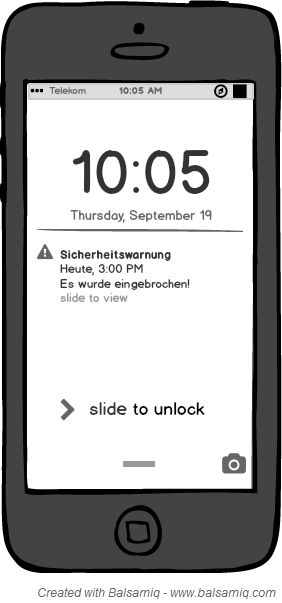
\includegraphics[scale=0.5]{Bilder/alert}
	\caption{Mockup einer Push-Benachrichtigung}
	\label{f:alert}
\end{figure}

Die Push-Benachrichtigung ist ein zentraler applikationsübergreifender Kommunikationskanal mobiler Geräte. Dabei wird die Kommunikation nicht vom Client (Smartphone / Tablet) initiiert, sondern von einem Server des Herstellers. Auf diese Weise ist es möglich, dem Besitzer des Sicherheitssystems ohne sein Zutun eine Nachricht zu übermitteln. Diese kann einen Text oder Link enthalten.\\
Durch die Verwendung von Push-Benachrichtigungen kann das Smartphone des Besitzers angewiesen werden, eine App des Sicherheitssystems zu öffnen und die aktuellen Meldungen anzuzeigen. Ebenfalls ist es denkbar, dass der Benutzer nach dem Empfang der Push-Benachrichtigung automatisch eine vom Sicherheitssystem erstellte Webseite öffnet, auf der er Bilder oder Videos des Einbruchs ansehen kann.



Da die Push-Benachrichtigung die modernste Form der Benachrichtigungen darstellt, ist die Verbreitung noch relativ gering. Mit modernen Mitteln ist sie jedoch leicht zu implementieren.
Da die Push-Systeme der verschiedenen mobilen Betriebssysteme technologisch unterschiedlich aufgebaut sind, sollte eine Plattformübergreifende Lösung eingesetzt werden.
Hierfür gibt es Dienste wie 'Pushover', die für mehrere Smartphone Betriebssysteme Anwendungen bereitstellen, die Push-Notifications empfangen können.
Mithilfe einer serverseitigen HTTP API ermöglicht Pushover das Senden von Push-Benachrichtigungen an zuvor angemeldete Gruppen oder Einzelgeräte. Um Nachrichten empfangen zu können müssen die Endgeräte die Pushover Application installiert haben, die für Android-, iOS- und Desktopcomputer erhältlich ist.

\vspace{5 mm}
\begin{figure}[H] 
	\centering
	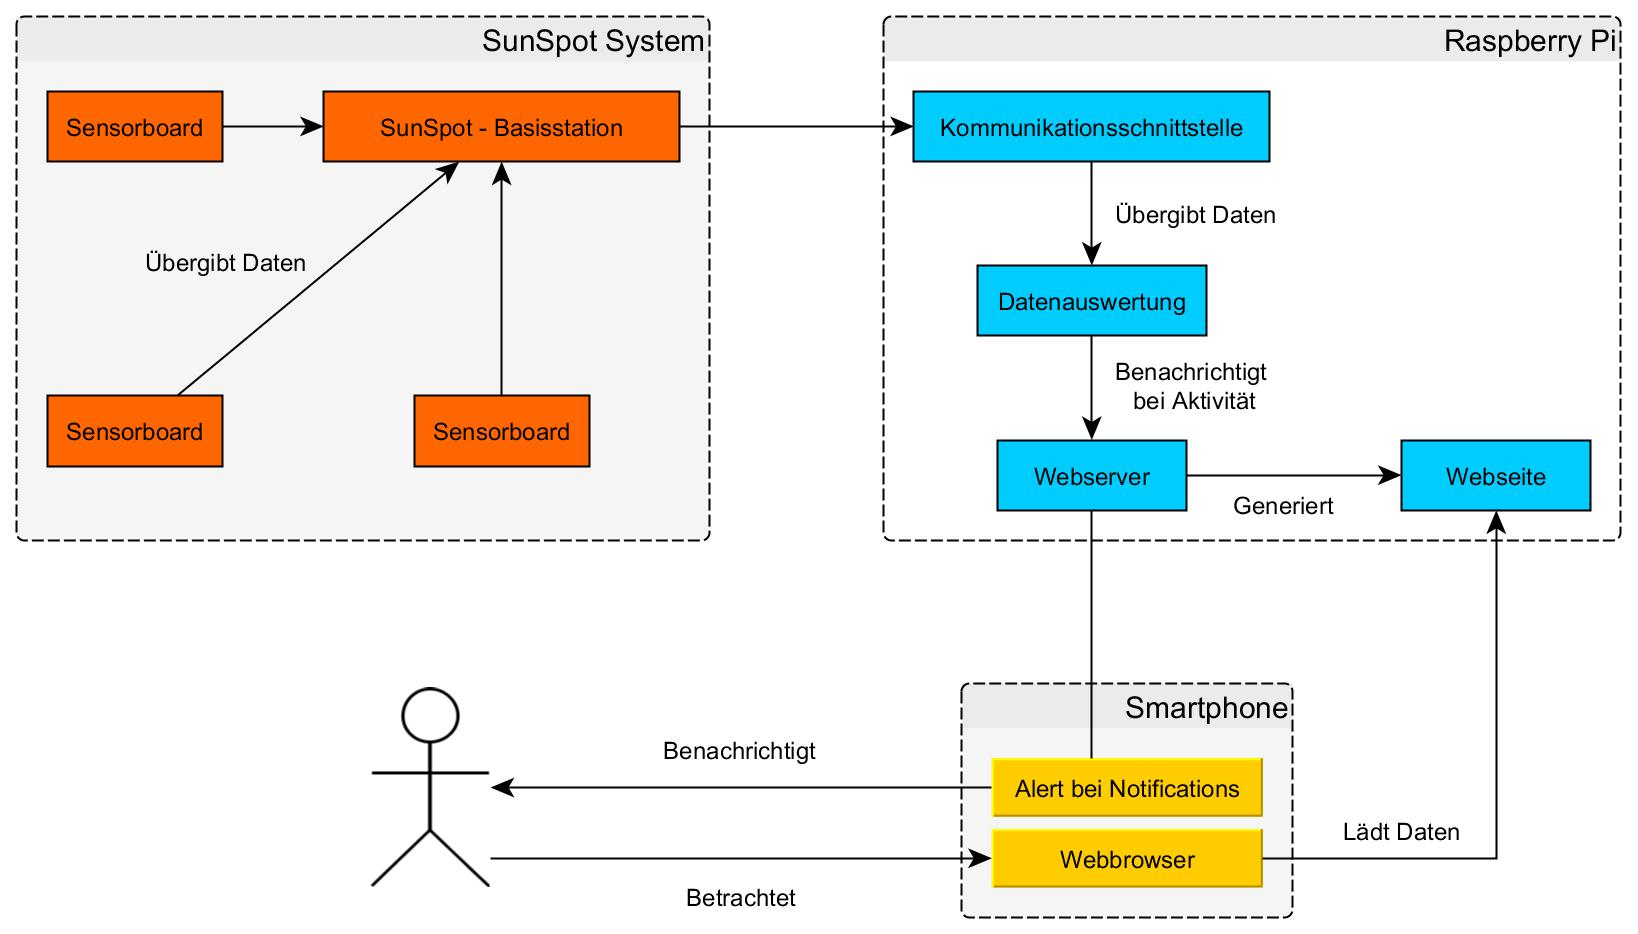
\includegraphics[scale=0.25]{Bilder/benachrichtigung}
	\caption{Aufbau eines Benachrichtigungssystems}
	\label{f:benachrichtigung}
\end{figure}

Die zu versendenden Nachrichten müssen an die HTTP API übergeben werden. Hierfür stellt Pushover bereits Codeausschnitte für eine Vielzahl von Geräten bereit.
Von einem Raspberry Pi, der im Beispielaufbau in Abbildung \ref{f:benachrichtigung} enthalten ist, können Pushover-Nachrichten per Kommandozeile an die API übergeben werden. 

\begin{lstlisting}[language=sh,caption={Beispielcode zum Senden einer Pushover-Nachricht},label=lst:pushovermsg,frame=single] 
curl -s \
--form-string "token=abc123" \
--form-string "user=user123" \
--form-string "message=hello world" \
https://api.pushover.net/1/messages.json
\end{lstlisting}


